
\vspace{0.15cm}
\begin{flushleft}
	{\color{blue!50!green}\fbox{\fontfamily{qag}\bfseries\selectfont PHẦN I. Câu trắc nghiệm nhiều phương án lựa chọn (3,0 điểm)}}
	\textit{\small (Thí sinh trả lời từ câu 1 đến câu 12. Mỗi câu hỏi thí sinh chỉ chọn một phương án.)}
\end{flushleft}
\setcounter{ex}{0}
\setcounter{bt}{0}

% Câu 1
\begin{ex}
	\macau{ID: VL10-BTX207-C01}Trong hệ đơn vị SI, đơn vị của gia tốc là
	\choice
	{$\text{m}\cdot\text{s}^2$}
	{$\text{m}\cdot\text{s}$}
	{$\text{m}\cdot\text{s}^{-1}$}
	{\True $\text{m}\cdot\text{s}^{-2}$}
	\loigiai{
		Đơn vị của gia tốc trong hệ SI là mét trên giây bình phương: $\text{m/s}^2 = \text{m}\cdot\text{s}^{-2}$.\par
	}
\end{ex}

% Câu 2
\begin{ex}
	\macau{ID: VL10-BTX207-C02}Đồng hồ đo thời gian hiện số MC964 khi đặt ở chế độ MODE A $+$ B dùng để
	\choice
	{đo thời gian vật chắn cổng quang điện nối với ổ B}
	{\True đo tổng hai khoảng thời gian vật chắn cổng quang điện nối với ổ A và cổng quang điện nối với ổ B}
	{đo thời gian vật chuyển động từ cổng quang điện nối với ổ A tới cổng quang điện nối với ổ B}
	{đo thời gian vật chắn cổng quang điện nối với ổ A}
	\loigiai{
		Ở chế độ MODE A $+$ B, đồng hồ đo tổng thời gian vật chắn cổng quang A và thời gian vật chắn cổng quang B: $\Delta t = \Delta t_A + \Delta t_B$.\par
	}
\end{ex}

% Câu 3
\begin{ex}
	\macau{ID: VL10-BTX207-C03}Chọn phát biểu đúng về vận tốc.
	\choice
	{Vận tốc là đại lượng vô hướng, luôn có giá trị không âm}
	{Vận tốc là đại lượng vectơ, có hướng ngược với hướng của độ dịch chuyển}
	{Vận tốc là đại lượng vô hướng, có thể nhận giá trị âm hoặc dương}
	{\True Vận tốc là đại lượng vectơ, có hướng trùng với hướng của độ dịch chuyển}
	\loigiai{
		Vận tốc $\vec{v} = \dfrac{\vec{d}}{\Delta t}$ là đại lượng vectơ; vì $\Delta t > 0$ nên $\vec{v}$ cùng hướng với độ dịch chuyển $\vec{d}$.\par
	}
\end{ex}

% Câu 4
\begin{ex}
	\macau{ID: VL10-BTX207-C04}Đối tượng nghiên cứu của Vật lí là
	\choice
	{\True các dạng vận động của vật chất và năng lượng}
	{sự phát triển sinh học của vật chất hữu cơ}
	{sự hình thành và phát triển của các lí thuyết vật lí}
	{cuộc đời và sự nghiệp của các nhà vật lí}
	\loigiai{
		Vật lí nghiên cứu các dạng vận động của vật chất (cơ, nhiệt, điện, từ, quang, hạt nhân,\ldots) và năng lượng.\par
	}
\end{ex}

% Câu 5
\begin{ex}
	\macau{ID: VL10-BTX207-C05}Chuyển động nào sau đây được coi là rơi tự do?
	\choice
	{Vận động viên đang nhảy dù từ máy bay xuống}
	{\True Viên sỏi nhỏ được thả rơi từ trên cao trong không khí}
	{Chiếc lá khô đang rơi từ trên cành xuống}
	{Sợi chỉ mảnh được thả rơi trong không khí}
	\loigiai{
		Vật được coi là rơi tự do khi lực cản của không khí rất nhỏ so với trọng lượng. Viên sỏi nhỏ, nặng thỏa mãn điều kiện này; dù, lá khô, sợi chỉ chịu lực cản lớn.\par
	}
\end{ex}

% Câu 6
\begin{ex}
	\macau{ID: VL10-BTX207-C06}Phát biểu nào sau đây về chuyển động thẳng biến đổi đều là \textbf{sai}?
	\choice
	{Trong chuyển động nhanh dần đều, vectơ gia tốc cùng chiều với chiều chuyển động}
	{Trong chuyển động thẳng biến đổi đều, gia tốc không đổi theo thời gian}
	{\True Trong chuyển động chậm dần đều, gia tốc luôn có giá trị âm}
	{Trong chuyển động chậm dần đều, vectơ gia tốc ngược chiều với chiều chuyển động}
	\loigiai{
		Trong chuyển động chậm dần đều, $\vec{a}$ ngược chiều $\vec{v}$ (tức $a \cdot v < 0$). Nếu vật chuyển động theo chiều âm ($v < 0$) thì $a > 0$. Vậy khẳng định gia tốc ``luôn có giá trị âm'' là sai.\par
	}
\end{ex}

% Câu 7
\begin{ex}
	\macau{ID: VL10-BTX207-C07}Gọi $\overline{A}$ là giá trị trung bình, $\Delta A'$ là sai số dụng cụ, $\overline{\Delta A}$ là sai số ngẫu nhiên và $\Delta A = \overline{\Delta A} + \Delta A'$ là sai số tuyệt đối của phép đo đại lượng $A$. Sai số tỉ đối của phép đo là
	\choice
	{$\delta A = \dfrac{\overline{\Delta A}}{\overline{A}} \cdot 100\%$}
	{$\delta A = \dfrac{\overline{A}}{\overline{\Delta A}} \cdot 100\%$}
	{$\delta A = \dfrac{\Delta A'}{\overline{A}} \cdot 100\%$}
	{\True $\delta A = \dfrac{\Delta A}{\overline{A}} \cdot 100\%$}
	\loigiai{
		Sai số tỉ đối bằng tỉ số giữa sai số tuyệt đối (toàn phần) và giá trị trung bình: $\delta A = \dfrac{\Delta A}{\overline{A}} \cdot 100\%$.\par
	}
\end{ex}

% Câu 8
\begin{ex}
	\macau{ID: VL10-BTX207-C08}Đồ thị độ dịch chuyển -- thời gian $(d - t)$ của chuyển động thẳng đều có dạng là
	\choice
	{\True đường thẳng}
	{đường tròn}
	{đường hypebol}
	{đường parabol}
	\loigiai{
		Chuyển động thẳng đều có $d = vt$ là hàm bậc nhất của $t$ nên đồ thị $(d - t)$ là một đường thẳng.\par
	}
\end{ex}

% Câu 9
\begin{ex}
	\macau{ID: VL10-BTX207-C09}Một vật chuyển động thẳng biến đổi đều với vận tốc ban đầu $v_0$, sau thời gian $t$ vật có vận tốc $v$. Gia tốc của vật là
	\choice
	{$a = \dfrac{v_0 - v}{t}$}
	{$a = \dfrac{v_0 + v}{t}$}
	{$a = \dfrac{v^2 - v_0^2}{t}$}
	{\True $a = \dfrac{v - v_0}{t}$}
	\loigiai{
		Theo định nghĩa: $a = \dfrac{\Delta v}{\Delta t} = \dfrac{v - v_0}{t}$.\par
	}
\end{ex}

% Câu 10
\begin{ex}
	\macau{ID: VL10-BTX207-C10}Một chất điểm đi được quãng đường $s$ trong khoảng thời gian $\Delta t$. Tốc độ trung bình của chất điểm là
	\choice
	{$v_{\text{tb}} = s \cdot \Delta t$}
	{$v_{\text{tb}} = s - \Delta t$}
	{\True $v_{\text{tb}} = \dfrac{s}{\Delta t}$}
	{$v_{\text{tb}} = \dfrac{\Delta t}{s}$}
	\loigiai{
		Tốc độ trung bình bằng quãng đường chia thời gian: $v_{\text{tb}} = \dfrac{s}{\Delta t}$.\par
	}
\end{ex}

% Câu 11
\begin{ex}
	\macau{ID: VL10-BTX207-C11}Độ dịch chuyển của một vật cho biết
	\choice
	{\True độ dài và hướng của sự thay đổi vị trí của vật}
	{vị trí và thời điểm chuyển động của vật}
	{mức độ nhanh hay chậm của chuyển động}
	{tổng độ dài quãng đường mà vật đã đi được}
	\loigiai{
		Độ dịch chuyển $\vec{d}$ là vectơ nối vị trí đầu với vị trí cuối, cho biết độ dài (khoảng cách thẳng) và hướng của sự thay đổi vị trí của vật.\par
	}
\end{ex}

% Câu 12
\begin{ex}
	\macau{ID: VL10-BTX207-C12}Khi phòng thực hành xảy ra sự cố cháy, hành động nào sau đây là \textbf{sai}?
	\choice
	{Ngắt ngay toàn bộ nguồn điện của phòng thực hành}
	{Di chuyển nhanh các chai lọ hóa chất, vật liệu dễ cháy ra khu vực an toàn}
	{Không dùng bình khí $\text{CO}_2$ để dập đám cháy trên quần áo người hoặc đám cháy kim loại kiềm}
	{\True Dùng nước dội trực tiếp để dập đám cháy ở nơi có thiết bị điện đang cắm nguồn}
	\loigiai{
		Nước dẫn điện, dội nước vào đám cháy có thiết bị điện đang cắm nguồn có thể gây chập điện, điện giật cho người chữa cháy. Đây là hành động sai.\par
	}
\end{ex}

\vspace{0.15cm}
\begin{flushleft}
	{\color{blue!50!green}\fbox{\fontfamily{qag}\bfseries\selectfont PHẦN II. Câu trắc nghiệm đúng sai (2,0 điểm)}}
	\textit{\small (Thí sinh trả lời từ câu 1 đến câu 2. Trong mỗi ý a), b), c), d) ở mỗi câu, thí sinh chọn đúng hoặc sai.)}
\end{flushleft}
\setcounter{ex}{0}
\setcounter{bt}{0}

% Phần II Câu 1
\begin{ex}
	\macau{ID: VL10-BTX207-C13}Một bạn học sinh đạp xe từ cổng trường THPT Chuyên Quốc Học Huế đi thẳng theo đường Lê Lợi $1\text{ km}$, sau đó rẽ phải vào đường Hùng Vương đi thẳng $500\text{ m}$ để đến quán chè Hẻm như sơ đồ hình bên. Coi hai đoạn đường vuông góc với nhau.
	\begin{center}
		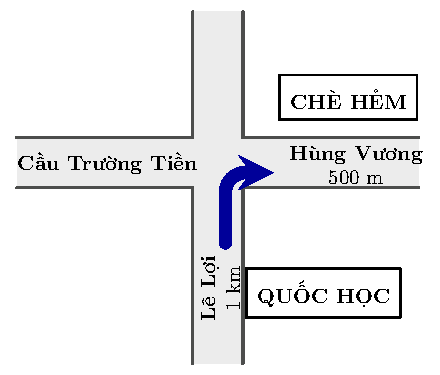
\includegraphics[width=5.6cm]{fig_cau13.pdf}
	\end{center}
	\choiceTF[t]
	{\True Quãng đường đi được và độ lớn độ dịch chuyển của bạn học sinh là khác nhau.}
	{Độ dịch chuyển của bạn học sinh là một đại lượng vô hướng.}
	{\True Quãng đường bạn học sinh đã đi được là $1{,}5\text{ km}$.}
	{Độ lớn độ dịch chuyển của bạn học sinh bằng $1180\text{ m}$.}
	\loigiai{
		{\color{green!50!black}\textbf{a) Đúng.}} Đường đi gấp khúc (có rẽ) nên quãng đường lớn hơn độ lớn độ dịch chuyển.\par
		{\color{red!80!black}\textbf{b) Sai.}} Độ dịch chuyển là đại lượng vectơ, có cả độ lớn và hướng.\par
		{\color{green!50!black}\textbf{c) Đúng.}} $s = 1000 + 500 = 1500\text{ m} = 1{,}5\text{ km}$.\par
		{\color{red!80!black}\textbf{d) Sai.}} Hai đoạn vuông góc: $d = \sqrt{1000^2 + 500^2} \approx 1118\text{ m} \ne 1180\text{ m}$.\par
	}
\end{ex}

% Phần II Câu 2
\begin{ex}
	\macau{ID: VL10-BTX207-C14}Một vật chuyển động thẳng dọc theo trục $Ox$ có phương trình độ dịch chuyển $d = 4t - t^2$ ($d$ tính bằng m, $t$ tính bằng s, $t \ge 0$).
	\choiceTF[t]
	{Vật chuyển động thẳng nhanh dần đều trong suốt quá trình chuyển động.}
	{\True Ngay sau thời điểm $t = 0$, vật chuyển động theo chiều dương của trục $Ox$.}
	{Gia tốc của vật bằng $1\text{ m/s}^2$.}
	{\True Vận tốc của vật tại thời điểm $t = 1\text{ s}$ bằng $2\text{ m/s}$.}
	\loigiai{
		{\color{red!80!black}\textbf{a) Sai.}} So sánh với $d = v_0t + \dfrac{1}{2}at^2$: $v_0 = 4\text{ m/s}$, $a = -2\text{ m/s}^2$. Ban đầu $a \cdot v_0 < 0$ nên vật chuyển động chậm dần đều (đến $t = 2\text{ s}$ thì đổi chiều).\par
		{\color{green!50!black}\textbf{b) Đúng.}} $v_0 = 4\text{ m/s} > 0$ nên ban đầu vật chuyển động theo chiều dương.\par
		{\color{red!80!black}\textbf{c) Sai.}} $a = -2\text{ m/s}^2 \ne 1\text{ m/s}^2$.\par
		{\color{green!50!black}\textbf{d) Đúng.}} $v = v_0 + at = 4 - 2t \Rightarrow v(1) = 4 - 2 \cdot 1 = 2\text{ m/s}$.\par
	}
\end{ex}

\vspace{0.15cm}
\begin{flushleft}
	{\color{blue!50!green}\fbox{\fontfamily{qag}\bfseries\selectfont PHẦN III. Câu trắc nghiệm trả lời ngắn (2,0 điểm)}}
	\textit{\small (Thí sinh trả lời từ câu 1 đến câu 4.)}
\end{flushleft}
\setcounter{ex}{0}
\setcounter{bt}{0}

% Phần III Câu 1
\begin{ex}
	\macau{ID: VL10-BTX207-C15}Tại giải vô địch điền kinh thế giới ở Berlin (Đức), vận động viên Usain Bolt lập kỉ lục thế giới chạy $100\text{ m}$ với thời gian $9{,}58\text{ s}$. Tốc độ trung bình của Usain Bolt trên đường chạy đó là bao nhiêu $\text{m/s}$? (Làm tròn kết quả đến chữ số hàng phần mười).

	\par\shortans[oly]{10,4}
	\loigiai{
		\[v_{\text{tb}} = \frac{s}{\Delta t} = \frac{100}{9{,}58} \approx 10{,}44 \approx 10{,}4\text{ m/s}.\]
	}
\end{ex}

% Phần III Câu 2
\begin{ex}
	\macau{ID: VL10-BTX207-C16}Hình bên là đồ thị độ dịch chuyển -- thời gian $(d - t)$ của một ô tô chuyển động thẳng. Vận tốc của ô tô bằng bao nhiêu $\text{m/s}$?
	\begin{center}
		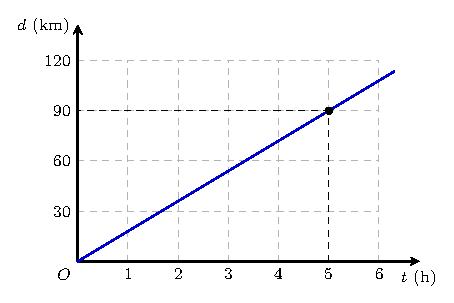
\includegraphics[width=5.6cm]{fig_cau16.pdf}
	\end{center}

	\par\shortans[oly]{5}
	\loigiai{
		Đồ thị là đường thẳng qua gốc tọa độ nên ô tô chuyển động thẳng đều. Tại $t = 5\text{ h}$ thì $d = 90\text{ km}$:\par
		\[v = \frac{d}{t} = \frac{90}{5} = 18\text{ km/h} = \frac{18}{3{,}6} = 5\text{ m/s}.\]
	}
\end{ex}

% Phần III Câu 3
\begin{ex}
	\macau{ID: VL10-BTX207-C17}Một người đang lái xe máy với tốc độ $28{,}8\text{ km/h}$ thì nhìn thấy một cái hố trước mặt nên hãm phanh, xe chuyển động chậm dần đều và dừng lại sau $5\text{ s}$. Chọn chiều dương là chiều chuyển động. Gia tốc của xe là bao nhiêu $\text{m/s}^2$?

	\par\shortans[oly]{-1,6}
	\loigiai{
		$v_0 = 28{,}8\text{ km/h} = 8\text{ m/s}$; $v = 0$.\par
		\[a = \frac{v - v_0}{\Delta t} = \frac{0 - 8}{5} = -1{,}6\text{ m/s}^2.\]
	}
\end{ex}

% Phần III Câu 4
\begin{ex}
	\macau{ID: VL10-BTX207-C18}Một vật được thả rơi tự do từ độ cao $80\text{ m}$ so với mặt đất. Lấy $g = 10\text{ m/s}^2$. Thời gian rơi của vật là bao nhiêu giây?

	\par\shortans[oly]{4}
	\loigiai{
		\[h = \frac{1}{2}gt^2 \Rightarrow t = \sqrt{\frac{2h}{g}} = \sqrt{\frac{2 \cdot 80}{10}} = 4\text{ s}.\]
	}
\end{ex}

\vspace{0.15cm}
\begin{flushleft}
	{\color{blue!50!green}\fbox{\fontfamily{qag}\bfseries\selectfont PHẦN IV. Tự luận (3,0 điểm)}}
	\textit{\small (Thí sinh trình bày lời giải từ câu 1 đến câu 3.)}
\end{flushleft}
\setcounter{ex}{0}
\setcounter{bt}{0}

% Phần IV Câu 1
\begin{ex}
	\macau{ID: VL10-BTX207-C19}Lúc 7 giờ, một ô tô chuyển động thẳng đều với tốc độ $40\text{ km/h}$ đi từ $A$ qua $B$ đến $C$. Biết $AB = 30\text{ km}$, $BC = 70\text{ km}$ ($A$, $B$, $C$ thẳng hàng theo thứ tự đó). Chọn gốc tọa độ tại $A$, chiều dương từ $A$ đến $B$, gốc thời gian lúc 7 giờ. Vẽ đồ thị độ dịch chuyển -- thời gian $(d - t)$ của ô tô.
	\loigiai{
		Phương trình độ dịch chuyển: $d = vt = 40t$ ($d$: km, $t$: h).\par
		-- Tại $A$: $t = 0$, $d = 0$.\par
		-- Tại $B$: $d_B = 30\text{ km} \Rightarrow t_B = \dfrac{30}{40} = 0{,}75\text{ h}$ (lúc 7 giờ 45 phút).\par
		-- Tại $C$: $d_C = 30 + 70 = 100\text{ km} \Rightarrow t_C = \dfrac{100}{40} = 2{,}5\text{ h}$ (lúc 9 giờ 30 phút).\par
		Đồ thị là đoạn thẳng đi qua $O(0; 0)$, $B(0{,}75; 30)$ và kết thúc tại $C(2{,}5; 100)$:\par
	\begin{center}
		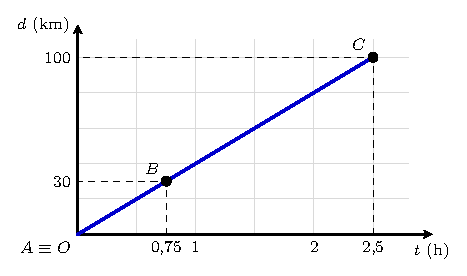
\includegraphics[width=7.0cm]{fig_cau19_giai.pdf}
	\end{center}
	}
\end{ex}

% Phần IV Câu 2
\begin{ex}
	\macau{ID: VL10-BTX207-C20}Một vật chuyển động thẳng biến đổi đều dọc theo trục $Ox$ có đồ thị vận tốc -- thời gian $(v - t)$ như hình bên. Tính:
	\par \textbf{a)} Gia tốc của vật. \par \textbf{b)} Quãng đường vật đi được trong $10\text{ s}$ đầu tiên.
	\begin{center}
		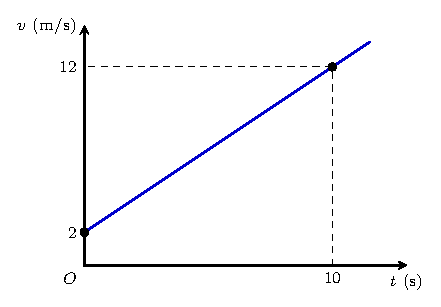
\includegraphics[width=5.2cm]{fig_cau20.pdf}
	\end{center}
	\loigiai{
		\textbf{a)} Từ đồ thị: $v_0 = 2\text{ m/s}$, tại $t = 10\text{ s}$ thì $v = 12\text{ m/s}$.\par
		\[a = \frac{v - v_0}{t} = \frac{12 - 2}{10} = 1\text{ m/s}^2.\]
		\textbf{b)} Vật chuyển động theo một chiều ($v > 0$) nên quãng đường bằng độ dịch chuyển:\par
		\[s = v_0t + \frac{1}{2}at^2 = 2 \cdot 10 + \frac{1}{2} \cdot 1 \cdot 10^2 = 70\text{ m}.\]
		(Hoặc tính diện tích hình thang dưới đồ thị: $s = \dfrac{(2 + 12) \cdot 10}{2} = 70\text{ m}$.)\par
	}
\end{ex}

% Phần IV Câu 3
\begin{ex}
	\macau{ID: VL10-BTX207-C21}Thả rơi tự do một vật từ độ cao $100\text{ m}$ so với mặt đất. Lấy $g = 10\text{ m/s}^2$. Tính:
	\par \textbf{a)} Quãng đường vật rơi được sau $3\text{ s}$ kể từ lúc thả. \par \textbf{b)} Độ cao của vật so với mặt đất tại thời điểm đó.
	\loigiai{
		\textbf{a)} \[s = \frac{1}{2}gt^2 = \frac{1}{2} \cdot 10 \cdot 3^2 = 45\text{ m}.\]\par
		\textbf{b)} Độ cao của vật so với mặt đất: $h' = h - s = 100 - 45 = 55\text{ m}$.\par
	}
\end{ex}
